\chapter{Future Work}
\label{chapter:future_work}

The contributions of this dissertation leave three complementary questions open: (1) how to divide DRAM between the DH and the I/O cache for SH, (2) how to select objects for migration to SH without application hints, and (3) how to reclaim SH space occupied by partially live regions.
This chapter proposes directions for addressing these questions, distinguishing extensions of the evaluated systems from mechanisms that require further design and validation.

\section{Applying FlexHeap to Storage-Backed Heaps}
\label{sec:future_flexheap}

An open direction is to apply \flexheapName{}'s I/O-aware heap sizing to Chipper, which uses G1.
Within a fixed DRAM budget, a larger DH can reduce collection pressure but leave less memory for caching SH pages and application files.
A smaller DH can increase cache capacity, but may also increase collection frequency and, depending on Chipper's placement and collection policies, migration activity.
The question is whether dynamically resizing DH improves this tradeoff as allocation rates and access patterns change; this integration has not been evaluated.
If effective, this approach could make storage-backed heaps easier to deploy by allowing the runtime to adjust the DH-I/O cache split, rather than requiring users to choose that division in advance within the configured DRAM budget.

FlexHeap would reclaim DRAM from DH for the OS I/O cache, but G1 can return only free regions to the OS.
If DH lacks enough free regions, G1 must first collect to create them, while retaining sufficient regions for allocation and evacuation.
This pressure to free regions may cause Chipper to collect earlier and, under its existing policy, migrate objects to SH sooner; the resulting SSD writes and access costs could affect application performance.
Changes in I/O cache capacity may also alter the estimated cost of evacuating candidate regions to SH and therefore affect G1's region-selection decisions.
An initial design should resize DH while retaining Chipper's existing placement policy, then evaluate coordinated resizing and migration separately.
Evaluation should compare Chipper's integrated configuration with its original configuration and fixed DH sizes under the same total memory budget, across workload phase changes.
It should measure throughput, application tail latency, GC pauses, device traffic, and DH, SH page-cache, and other cached-memory residency separately.
Lower aggregate GC and I/O costs alone would not show that Chipper still meets application latency requirements; tail latency should also be assessed against an application target where one is defined.

\section{Automatic Selection of Objects for the Storage-Backed Heap}
\label{sec:future_placement}

TeraHeap and Chipper rely on framework hints to guide migration to SH.
A hint identifies a root whose reachable objects are candidates for movement, signals when the application considers the data ready to move, and assigns a label to co-locate objects with similar expected lifetimes.
Co-location can support region-level reclamation, but does not guarantee that all objects in a group become unreachable together.
This approach requires framework modifications and may not be practical for unfamiliar applications.

\begin{figure}[t]
	\centering
	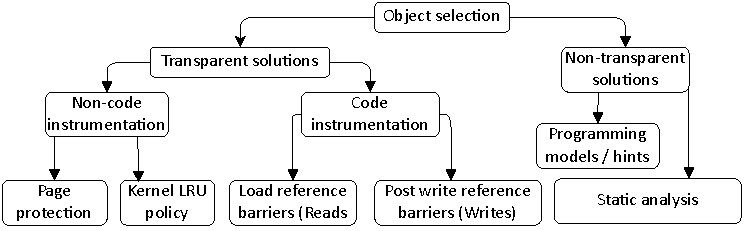
\includegraphics[width=0.9\linewidth]{future_work/fig/object_selection_taxonomy.pdf}
	\caption{Taxonomy of approaches for selecting objects to move from a fast to a slow memory tier, adapted from the GateKeeper related-work taxonomy.}
	\label{fig:future_object_selection}
\end{figure}

Prior work explores both application-visible and transparent placement decisions (Figure~\ref{fig:future_object_selection}).
Application-visible approaches use hints, programming models, or static analysis to identify candidates, as in TeraHeap, JPDHeap, and Panthera~\cite{teraheap,jpd_heap,wang:Panthera}.
Transparent approaches infer placement from runtime instrumentation, staleness profiles, or operating-system page-replacement policies.
Write-Rationing, GCMove, and ThinGC instrument accesses, while Sleigh and LeakSurvivor profile object staleness~\cite{akram:ration,gcmove,thingc,bond:sleigh,leaksurvivor}; Semeru, MemLiner, and Mako rely on kernel LRU policies to manage data across memory tiers~\cite{wang:semeru,wang:memliner,ma:mako}.
These approaches differ in application effort, selection precision, and monitoring overhead.
For storage-backed heaps, the challenge is to obtain useful object-level placement information without monitoring costs that outweigh its benefits.

We initially tried Intel PEBS load-latency sampling to identify cold objects without application hints, but it produced many false-positive candidates because it reports process memory addresses rather than Java object identities, and accesses to thread stacks, JIT/runtime metadata, and other non-heap memory complicate attribution~\cite{intel:pebs_events}.
This result makes PEBS alone an unreliable signal for identifying cold heap objects, particularly as GC evacuation and address reuse change object locations.

A longer-term goal is to infer the hint decisions from runtime observations, which would require additional access and reference metadata beyond the information the JVM already collects.
One proposal is to instrument selected field and array loads in hot methods compiled by C2, setting an access bit for the object whose contents are read.
At the end of each G1 concurrent-mark cycle, the runtime could combine these bits with G1's marked-object information to update per-object hotness and cold-streak estimates.
Objects with no recorded C2 access may still be accessed through the interpreter, C1-compiled code, intrinsics, or native code; C2-only observations therefore cannot establish that they are cold.
Likewise, loading a reference does not make the entire reachable object graph hot.
The runtime would need to preserve or transfer access history when G1 evacuates objects and distinguish mutator accesses from collector scans.
A read-only signal is insufficient to estimate mutation costs: rarely read but frequently updated objects may generate substantial SH traffic, and capturing these writes requires monitoring reference and primitive-field or array stores.

To group candidates, a concurrent phase could build connected components from references among objects classified as cold, using a union-find data structure.
This proposal requires a stable and sufficiently complete view of the reference graph; load observations alone do not provide one.
Mutators can update an object through a reference loaded earlier, so changes to object fields require separate write tracking and reconciliation with G1's concurrent-marking barriers.
After Remark, a phase could assign labels to validated groups that remain cold for several cycles, meet a minimum size, and have few references crossing group boundaries, especially incoming references from hot objects that could keep an SH region live.
The labels would guide co-location during migration, but would not guarantee that the entire group moves in one cycle or is reclaimed together.
G1 selects old regions for mixed collections according to its collection policy, so migration may span several cycles and some candidate regions may be deferred.
Partial migration can create references from SH objects to objects that remain in DH; the runtime must track, trace, and update these references, including when their SH source regions are not selected for collection.
A per-object check during evacuation could redirect recently accessed candidates to DH, provided the access updates are visible before the check and the evacuation path reserves sufficient DH space.

We expect the barrier to add little to execution time because it avoids most of its work.
First, it checks the target's region in a small table, one byte per region, that fits in the L1 cache.
Only objects in monitored old regions pass this check.
For young objects, H2 objects, and all objects while monitoring is off, the barrier costs a few instructions with predictable branches.
Second, for monitored objects the barrier stores the access bit only when it is not already set.
Each object therefore causes at most one header store per marking cycle, and cold objects, by definition, never trigger the barrier at all.
Third, the barrier uses no atomic instructions.
A race with the collector can only make an object look hotter than it is, never colder, so errors cost selection recall but never cause hot data to move to H2.
In addition, monitoring is enabled only when H1 is under memory pressure.
If checking the object header still proves too expensive for reference-heavy code, the access bits can move to a side table indexed by address, so the barrier never touches the object.
Measuring this overhead, and comparing transparent selection against hint-based selection as an oracle, is the main evaluation this work requires.

\section{Space Reclamation in the Storage Heap}
\label{sec:future_reclamation}

Whole-region reclamation avoids scanning storage-resident objects.
However, a small live subset can retain an otherwise dead region.
We designed SmartSweep~\cite{kolokasis:smartsweep} as a proof-of-concept for addressing this limitation: it estimates region garbage and transfers selected regions back to local memory for collection.
Its preliminary prototype moves only primitive arrays and leaf objects whose fields contain primitive values.
Consequently, it does not implement the general case in which SH objects contain references to DH or to other SH regions.
Extending this approach to arbitrary object graphs requires both useful garbage estimates and a reference-management protocol that remains correct as objects move.

A first research direction is to estimate garbage from changes in references and in each region's object graph without repeatedly scanning its objects on storage.
When objects enter SH, the runtime could construct DRAM-resident summaries of their sizes, entry points, and connectivity while the objects are already being processed.
Subsequent GC observations of DH-to-SH references and records of reference insertions and deletions could update these summaries.
For example, removing an entry point to a previously isolated subgraph could indicate that some of its bytes have become garbage.
However, another path may still reach that subgraph, and internal cycles can remain after all external paths disappear.
Reference counts or counts of changed edges therefore cannot, in general, establish the amount of unreachable data.
The research problem is to find summaries that predict reclaimable space accurately enough to guide selection while keeping metadata, write-barrier work, and any selective rescanning affordable.

Garbage estimates would rank regions for reclamation, not authorize the destruction of individual objects.
A conservative starting point would copy all objects from a selected region into DH and let the collector determine which are unreachable from the preserved incoming references.
This process still incurs reads and copies for garbage objects and requires temporary DH capacity.
Selection should therefore weigh expected reclaimed space against transfer cost, subsequent GC work, and reference-repair cost, with a bounded import budget.
Before imported objects are collected, incoming references from SH must be represented in the collector's root processing, including references from regions that are not themselves selected for reclamation.
Coarse region-dependency information may be insufficient to identify these object-level roots precisely.
Conservative retention can preserve correctness, but may delay the reclamation that the transfer was intended to enable.

A second research direction is to separate reuse of SH backing storage from reuse of its virtual addresses, allowing inter-region reference repair to proceed lazily.
The runtime could reserve a virtual address range for SH and map each active region to backing storage within this range.
As an initial design, the runtime would stop mutators while copying a selected region's contents to DH, publishing forwarding information in DRAM, and making the old virtual range inaccessible before releasing the corresponding backing extents for reuse.
Protecting a mapping alone does not release those extents; storage deallocation or reuse must be an explicit step.
The old virtual range would remain reserved so that dereferencing an obsolete address triggers a protection fault instead of accessing unrelated objects.
Forwarding information must identify object boundaries and destinations without reading the released storage.

A third challenge is to identify and repair the source fields that still point into an evacuated SH region.
Protecting the region's old virtual-address range makes a dereference of a stale pointer fault and reveals the old target address, which forwarding metadata can map to the object's DH copy.
The fault does not reveal which object field supplied that pointer, so compiled heap-field accesses would need to place the address of the source slot in a designated register for the fault handler.
The handler could use that slot address and the forwarding metadata to update the field, then resume the access using the forwarded address.
This approach would lazily repair SH references on access without adding a load barrier to every reference access, as barrier-based designs such as ZGC do~\cite{yang:zgc}.
It depends on the source slot remaining valid until repair and requires correct handling of concurrent faults, writes, and GC activity; roots held in registers or stacks also need a separate repair path.
Because aliases may remain stale until accessed, reference comparisons must preserve object-identity semantics even when one pointer has been repaired and another has not.
The cost of faulting accesses to unrelated objects that share a protected region, along with the compiler and runtime changes, must be evaluated.

Lazy repair must preserve object reachability as well as address validity.
The existing mechanism handles references from DH objects to SH objects.
The unresolved case is an SH field that still points to an object evacuated to DH: the DH collector must treat it as an edge to the object's current location, including after the object moves again.
Forwarding metadata and the old virtual-address range must remain available while stale pointers may still be dereferenced; otherwise, reusing the address could make a stale pointer refer to an unrelated object.
Treating every forwarding entry as a permanent GC root, however, would retain objects that are otherwise unreachable.
The runtime therefore needs to establish when no stale pointers can refer to an evacuated address before reclaiming its forwarding metadata and reusing that virtual address.
How to establish this safely in the presence of unaccessed SH fields, cycles, and concurrent GC remains an open question.
The design must also bound the virtual address space and metadata consumed while old addresses remain reserved.

Evaluation should extend beyond primitive-only objects to shared, cyclic, and mutable graphs with references in both directions between DH and SH.
It should measure garbage-estimation error, reclaimed backing capacity, transferred bytes, temporary DH demand, fault-induced latency, and metadata growth over long executions.
Comparisons with whole-region reclamation and eager reference repair would establish when delayed repair saves enough I/O to justify its additional complexity.
The broader question is how much liveness and reference information must be maintained in DRAM to reclaim storage promptly without repeatedly tracing the storage heap.
